\begin{tikzpicture}[remember picture]
    \node (light-node){
        
\includegraphics[scale = 0.05]{figs/icons/computer.eps}
    };
    \node[scale = 0.35,below=0cm of light-node] (light-label) {\textbf{Light Node}};

    \node (full-node) [matrix, below left = of light-node]{ 
        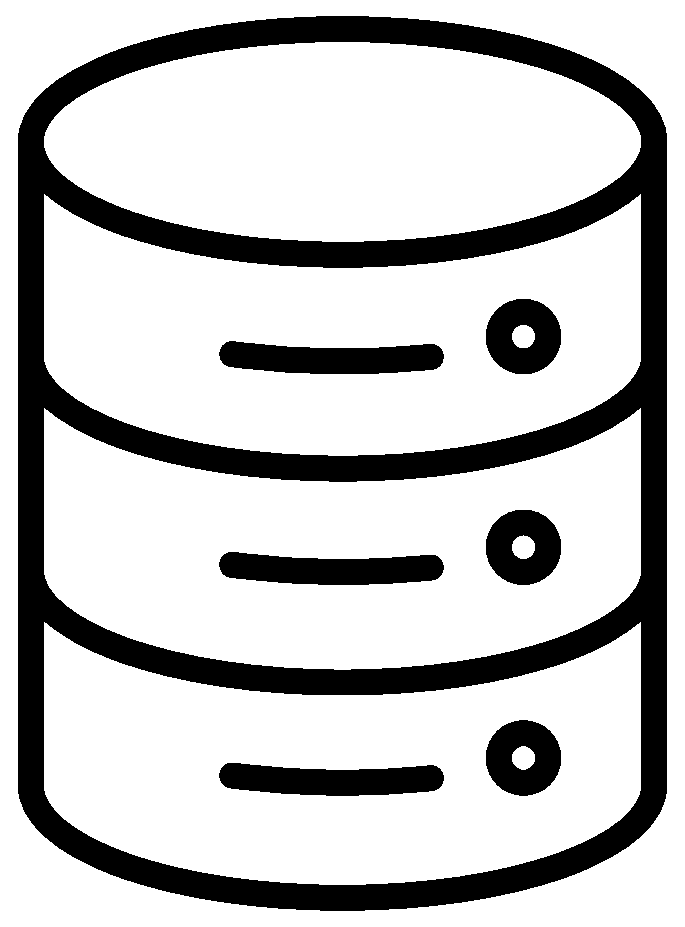
\includegraphics[scale = 0.05]{figs/icons/database.eps}
        \\
    };
    \node[scale = 0.35,below = 0cm of full-node,xshift=5ex] (full-label) {\textbf{Full Node}};

    \node (miner) [matrix, below right = 1.02cm and 0.5cm of light-node]{
        
\includegraphics[scale = 0.45]{figs/icons/server.eps}
        \\
    };
    \node[scale = 0.35,below = 0cm of miner,xshift=6.5ex] (miner-label) {\textbf{Miner}};

    \draw [->] (-0.45,-0.05) -- (-1.3,-0.85) 
    node [above,midway,sloped,scale=0.3]
    {Query};

    \draw [<-] (-0.38,-0.17) -- (-1.15,-0.9) 
    node [below,midway,sloped,scale=0.3]
    {Answers \& Proof};

    \draw  (-1.15,-1.2) -- (1.2,-1.2);

    \draw [->] (0.45,-0.05) -- (1.35,-0.8) 
    node [above,midway,sloped,scale=0.3]
    {Query};

    \draw [<-] (0.42,-0.17) -- (1.22,-0.82) 
    node [below,midway,sloped,scale=0.3]
    {Answers \& Proof};
\end{tikzpicture}